\documentclass[answers]{exam}

\usepackage{bm}
\usepackage{tikz}
\usepackage{pgfplots}
\usepackage{algpseudocode}

\pgfplotsset{compat=1.15}

\lhead{\textbf{CS109} Spring 2019}
\rhead{Problem Set 1}
\cfoot{\thepage}

\qformat{\textbf{Problem \thequestion.} \hfill}

\title{Problem Set 1}
\author{Andrew Li}
\date{}

\begin{document}
\maketitle

\begin{questions}
	% 1
	\question
	A substitution cipher is derived from an ordering of the letters in the alphabet. How many ways can the 26 letters be ordered if each letter appears exactly once and:
	\begin{parts}
		\part There are no other restrictions?
		\part The letters Q and U must be next to each other (but in any order)?
	\end{parts}

	% 1
	\begin{solution}
	\begin{parts}
		\part $\bm{26!}$ The first letter in the ordering could be one of 26 choices, the next 25, and so until the last letter is order. Thus we have $26 \cdot 25 \cdots 1 = 26!$.
		\part $\bm{2 \cdot 26 \cdot 24!}$ There are 2 ways to arrange Q and U. Next, there are 26 ways of ordering either Q or U first, then there is only 1 place to order the other. For the other 24 letters there remain $24!$ orderings.
	\end{parts}
	\end{solution}

	% 2
	\question You are counting cards in a card game that uses \textbf{four} standard decks of cards. There are 208 cards total. Each deck has 52 cards (13 values each with 4 suits). Cards are only distinguishable based on their suit and value, not which deck they came from.
	\begin{parts}
	\part In how many distinct ways can the cards be ordered?
	\part You are dealt two cards. How many distinct pairs of cards can you be dealt? Note: the order of the two cards you are dealt does not matter.
	\part You are dealt two cards. Cards with values 10, Jack, Queen, King and Ace are considered "good" cards. How many ways can you get two "good" cards? Order does not matter.
	\end{parts}

	% 2
	\begin{solution}
	\begin{parts}
		\part $\bm{208!/(4!)^{52}}$ There are $208!$ orderings assuming cards are distinguishable by deck. For each of the 52 cards, there are $4!$ ways of arranging the cards of same suit and value from all decks. So dividing by $52 \cdot 4!$ removes over-counting.
		\part $\bm{{52 \choose 2} + 4}$ There are 52 choose 2 ways to order two different cards in any way from the deck. Then adding 4 accounts for double card pairs since there are multiple decks.
		\part $\bm{{5 \choose 2} + 5}$ Again, you can choose two distinct cards in any order 5 choose 2 ways. Adding 5 accounts for double card pairs.
	\end{parts}
	\end{solution}
	
	% 3
	\question In how many ways can $n$ identical server requests ("identical balls") be distributed among $r$ servers ("urns") so that the $i$th server receives at least $m_i$ requests, for each $i = 1, 2, \dots, r$? You can assume that $n \geq \sum_{i=1}^r m_i$.
	
	\begin{solution}
	Let $m = \sum_{i=1}^r m_i$. Thus we have 
	\[\bm{{n - m + r - 1 \choose r - 1}}\]
	We must reserve $m$ requests in total for all servers. For the rest $n - m$ requests and $r - 1$ bars, we must choose $r - 1$ bars to split and distribute the rest. Thus $n - m + r - 1$ choose $r - 1$ gives us the number of distributions.
	\end{solution}
	
	% 4
	\question Determine the number of vectors $(x_1, x_2, \dots, x_n)$ such that each $x_i$ is a non-negative integer and $\sum_{i=1}^n x_i \leq k$, where $k$ is some constant non-negative integer. Note that you can think of $n$ (the size of the vector) as a constant that can be used in your answer.
	
	% 4
	\begin{solution}
	Suppose we have $k$ dots in an array:
	\begin{center}
		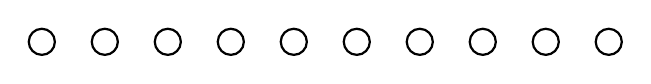
\begin{tikzpicture}
			\foreach \x in {0,...,9} {
				\node[thick,circle,draw] (\x) at (0.8 * \x + 0.4, 0.4) {};
			}
		\end{tikzpicture}
	\end{center}
	We can choose $n - 1$ dividers and assign each division length to $x_i$ for $i \in \{1, 2, \dots, n\}$. For $k = 10$, $n = 5$ one such construction is:
	\begin{center}
		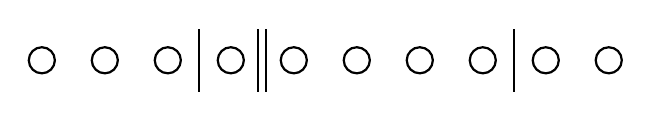
\begin{tikzpicture}
			\foreach \x in {0,...,9} {
				\node[thick,circle,draw] (\x) at (0.8 * \x + 0.4, 0.4) {};
			}
			
			\draw[thick] (3 * 0.8, 0) -- (3 * 0.8, 0.8);
			\draw[thick] (4 * 0.8 - 0.05, 0) -- (4 * 0.8 - 0.05, 0.8);
			\draw[thick] (4 * 0.8 + 0.05, 0) -- (4 * 0.8 + 0.05, 0.8);
			\draw[thick] (8 * 0.8, 0) -- (8 * 0.8, 0.8);
		\end{tikzpicture}
	\end{center}
	Thus $x_1 = 3$, $x_2 = 1$, $x_3 = 0$, $x_4 = 4$, and $x_5 = 2$. So the number of ways to satisfy $\sum_{i=1}^n x_i = k$ is equal to
	\[{k + n - 1 \choose n - 1}\]
	Iterating for all values $0, 1, \dots, k$, we have that the number of ways to satisfy $\sum_{i=1}^n x_i \leq k$ is equal to
	\[\bm{\sum_{i = 0}^k {i + n - 1 \choose n - 1}}\]
	\end{solution}
	
	% 5
	\question Imagine you have a robot ($\Theta$) that lives on an $n \times m$ grid:
	\begin{center}
	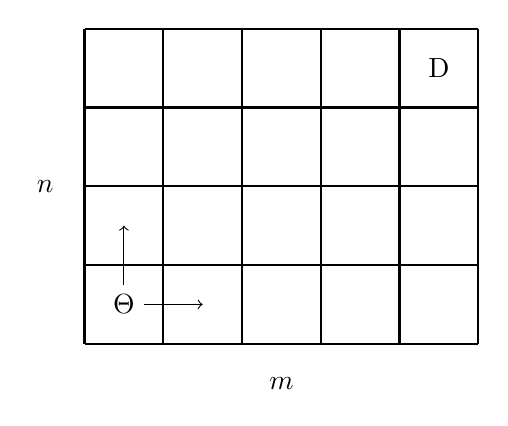
\begin{tikzpicture}
		\draw[step=1.0,black,thick,xshift=0.5cm,yshift=0.5cm] (0, 0) grid (5, 4);
		
		\node at (0, 2.5) (n) {$n$};
		\node at (3, 0) (m) {$m$};
		\node at (5, 4) (D) {D};
		\node at (1, 1) (R) {$\Theta$};
		
		\draw[->] (R) to (1, 2);
		\draw[->] (R) to (2, 1);
	\end{tikzpicture}
	\end{center}
	The robot starts in cell $(1, 1)$ and can take steps either to the right or up (no left or down steps). How many distinct paths can the robot take to the destination in cell $(n, m)$:
	\begin{parts}
		\part If there no additional constraints?
		\part The robot must start by moving to the right?
		\part If the robot changes direction exactly 3 times? As an example: moving up two times in a row is not changing directions but switching from moving up to moving right is. Moving [Up, Right, Right, Up] would count as having two direction switches.
	\end{parts}
	
	% 5
	\begin{solution}
		\begin{parts}
			\part $\bm{{n + m - 2 \choose n - 1}}$ An invariant for any sequence of moves is that the robot will take $(n - 1) + (m - 1)$ moves. Out of these $n + m - 2$ moves, we must have $m - 1$ right moves and $n - 1$ up moves necessarily which are each indistinguishable, thus we have:
			\[{n + m - 2 \choose n - 1} = {n + m - 2 \choose m - 1}\]
			\part $\bm{{n + m - 3 \choose n - 1}}$ If the robot starts by moving to the left, we have the same problem with dimension $n \times (m - 1)$. Thus we have
			\[{n + m - 3 \choose n - 1} = {n + m - 3 \choose m - 2}\]
			\part $\bm{{n + m - 3 \choose 3}}$ We can denote a direction change by a divider of a sequence of right and up moves. There are $n + m - 2$ moves and thus $n + m - 3$ dividers. Choosing three leads to the number of ways.
		\end{parts}
	\end{solution}
	
	% 6
	\question Given all the start-up activity going on in high-tech, you realize that applying combinatorics to investment strategies might be an interesting idea to pursue. Say you have \$20 million that must be invested among 4 possible companies. Each investment must be in integral units of \$1 million, and there are minimal investments that need to be made if one is to invest in these companies. The minimal investments are \$1, \$2, \$3, and \$4 million dollars, respectively for company 1, 2, 3, and 4. How many different investment strategies are available if
	\begin{parts}
		\part an investment must be made in each company?
		\part investments must be made in at least 3 of the 4 companies?
	\end{parts}
	
	% 6
	\begin{solution}
		\begin{parts}
			\part $\bm{{13 \choose 3}}$ Like Problem 3, except now there are 4 "buckets" (companies) and \$10 million is reserved, so only \$10 million is to be distributed to the four after minimal investments. 
			\part $\bm{{16 \choose 2} + {13 \choose 2} + {15 \choose 2} + {14 \choose 2} + {13 \choose 3}}$ We have 4 different ways of choose 3 companies: 123, 234, 124, 134. With casework, we can see that for 123, there are ${16 \choose 2}$ possibilities. For 234, there are ${13 \choose 2}$, 124 there are ${15 \choose 2}$, and for 134 there are ${14 \choose 2}$. The last possibility is to choose 4 companies, which has number of possible distributions determined in (a). Since all these different selections are mutually exclusive by the Sum Rule the solution follows.
		\end{parts}
	\end{solution}

	% 7
	\question If we assume that all possible poker hands (comprised of 5 cards from a standard 52 card deck) are equally likely, what is the probability of being dealt:
	\begin{parts}
		\part a flush? (A hand is said to be a flush if all 5 cards are of the same suit. Note that this definition means that \textit{straight flushes}--five cards of the same suit in numeric sequence--are also considered flushes.)
		\part one pair? (This occurs when the cards have numeric values $a, a, b, c, d$, where $a, b, c$ and $d$ are all distinct.)
		\part two pairs? (This occurs when the cards have numeric values $a, a, b, b, c$, where $a, b$ and $c$ are all distinct.)
		\part three of a kind? (This occurs when the cards have numeric values $a, a, a, b, c$, where $a, b$ and $c$ are all distinct.)
		\part four of a kind? (This occurs when the cards have numeric values $a, a, a, a, b$, where $a \neq b$.
	\end{parts}
	
	% 7
	\begin{solution}
		\begin{parts}
			\part $\bm{(12 \cdot 11 \cdot 10 \cdot 9)/(51 \cdot 50 \cdot 49 \cdot 48)}$ The first item card can be any card. The second must come from the same suit, which has already had one card removed, thus a $12/51$ chance. Repeating this for three more cards yields the solution.
			\part $\bm{4 \cdot 5!/2!}$ There are four ways of choose one of $a$, $b$, $c$, or $d$ to be repeated. There are then $5!$ ways to arrange the numbers, accounting for one repeat, thus $4 \cdot 5!/2!$ ways to choose one pair.
			\part $\bm{3 \cdot 5!/(2!)^2}$ There are three ways to choose two values from $a$, $b$ or $c$. Then for these five, there are $5!$ permutations to arrange them, dividing to account for 2 pairs of duplicates.  
			\part $\bm{3 \cdot 5!/3!}$ There are three ways to choose one values out of $a$, $b$, and $c$. Next, there are $5!/3!$ ways to arrange the five values with 3 indistinguishable values.
			\part $\bm{2 \cdot 5!/4!}$  There are two ways to choose one value from $a$ and $b$. For the five numbers, there are $5!/4!$ arrangements accounting for 4 indistinguishable values.
		\end{parts}
	\end{solution}
	
	% 8
	\question Say we roll a fair 6-sided die six times, what is the probability that we will roll:
	\begin{parts}
		\part three different numbers, twice each?
		\part some number \textit{exactly} 4 times?
	\end{parts}
	
	% 8
	\begin{solution}
		Assuming rolls are independent:
		\begin{parts}
			\part $\bm{25/648}$ There are ${6 \choose 3}$ ways of choosing 3 numbers. Next, construct 6 numbers, a pair of each number. There are $6!/(2!)^3$ of arranging these numbers since a pair is indistinguishable. So there are ${6 \choose 3} \cdot 6!/(2!)^3$ arrangements of three different numbers with twice of each. Dividing this by the number of possible arrangements of all six rolls, $6^6$, yields the probability.
			\part $\bm{1/216}$ $P(\textrm{same number 4 times}) = P(\textrm{any number}) \cdot P(\textrm{that same number})^3$. On the first roll, it can be any number. On subsequent trials, we have $1/6$ chance of rolling that same number again, thus $P(\textrm{same number 4 times}) = 1 \cdot (1/6)^3 = 1/216$.
		\end{parts}
	\end{solution}
	
	% 9
	\question To get good performance when working with binary search trees (BSTs), we must consider the probability of producing completely degenerate BSTs (where each node in the BST has at most one child).
	\begin{parts}
		\part If the integers 1 through $n$ are inserted in arbitrary order into a BST (where each possible order is equally likely), what is the probability (as an expression in terms of $n$) that the resulting BST will be completely degenerate?
		\part Using your expression from part (a), determine the smallest value of $n$ for which the probability of forming a completely degenerate BST is less than 0.01 (i.e., 1\%).
	\end{parts}
	
	% 9
	\begin{solution}
		\begin{parts}
			\part $\bm{2^{n-1}/n!}$ There are $n!$ ways to permute $1, 2, \dots, n$, which comprise the sample space. For $n$ integers, there are $2^{n-1}$ degenerate trees possible, as each node can choose a left or right child for its only child. The $n - 1$ power ensures the case works out for $n = 1$. Finally, the ratio between number of favorable outcomes and all outcomes is the probability.
			\part $\bm{8}$ By inspection, $2^6/7! \approx 0.013$ while $2^7/8! \approx 0.0032$.
		\end{parts}
	\end{solution}
	
	% 10
	\question Say a hacker has a list of $n$ distinct password candidates, only one of which will successfully log her into a secure system.
	\begin{parts}
		\part If she tries passwords from the list at random, deleting those passwords that do not work, what is the probability that her first successful login will be \textit{exactly} on her $k$th try?
		\part Now say the hacker tries passwords from the list at random, but does \textbf{not} delete previously tried passwords from the list. She stops after her first successful login attempt. What is the probability that her first successful login will be \textit{exactly} on her $k$th try?
	\end{parts}
	
	% 10
	\begin{solution}
		\begin{parts}
			\part 
			\[\bm{
				\left(\prod_{i=0}^{k - 2} \frac{n - i - 1}{n - i}\right) \frac{1}{n - k + 1} = 
					\underbrace{\frac{n - 1}{n} \cdot \frac{n - 2}{n - 1} \cdots \frac{n - k + 1}{n - k + 2} \cdot \frac{1}{n - k + 1}}_{\textrm{$k$ attempts}}
			}\]
			Each time she tries a password, she has a probability of $(m-1)/m$ of a successful login where $m$ is the number of passwords she has not eliminated yet. This number decreases by 1 after each login attempt, until the $k$th try, where she chooses the 1 correct password out of the $n - k + 1$ remaining.
			\part
			\[\bm{\frac{(n - 1)^{k - 1}}{n^k}}\]
			For the first $k - 1$ attempts, the probability is the same, $(n-1)/n$. On the $k$th try, there is a $1/n$ chance of successful login.
		\end{parts}
	\end{solution}
	
	% 11
	\question Say a university is offering 3 programming classes: one in Java, one in C++, and one in Python. The classes are open to any of the 100 students at the university. There are:
	\begin{enumerate}
		\item a total of 27 students in the Java class
		\item a total of 26 students in the C++ class
		\item a total of 18 students in the Python class
		\item 12 students in both the Java and C++ classes
		\item 5 students in both the Java and Python classes
		\item 7 students in both the C++ and Python classes
		\item 3 students in all three classes (note: these students are also counted as being in each pair of classes in the numbers above).
	\end{enumerate}
	\begin{parts}
		\part If a student is chosen randomly at the university, what is the probability that he or she is not in any of the 3 programming classes?
		\part If a student is chosen randomly at the university, what is the probability that he or she is taking \textit{exactly one} of the three programming classes?
		\part If two students are chosen randomly at the university, what is the probability that at least one of the chosen students is taking at least one programming class?
	\end{parts}
	
	% 11
	\begin{solution}
		\begin{parts}
			\part $\bm{56/100}$ The probability that a random student is not taking any of the 3 programming classes is the complement of the random student taking any of the classes. There are $27 + 26 + 18 - 12 - 5 - 7 - 3 = 44$ students taking any of the three, so there are 56 out of 100 that do not take any.
			\part $\bm{14/100}$ To find those solely in one class, subtract all overlapping students from the total for all classes. So for those only taking Java: $27 - 12 - 5 - 3 = 7$, C++: $26 - 12 - 7 - 3 = 4$, and Python: $18 - 5 - 7 - 3 = 3$. Thus we have $(7 + 4 + 3)/100$.
			\part $\bm{14/45}$ This is the complement of the event both do not take any programming courses. This has a probability $56/100 \cdot 55/99 = 14/45$ from (a).
		\end{parts}
	\end{solution}
	
	% 12
	\question A binary string containing $M$ 0's and $N$ 1's (in arbitrary order, where all orderings are equally likely) is sent over a network. What is the probability that the first $r$ bits of the received message contain exactly $k$ 1's?
	
	% 12
	\begin{solution}
		$\bm{{r \choose k}/{M + N \choose N}}$ There are ${M + N \choose N}$ ways to arrange the binary string, so the same amount for the first $r$ bits. There are ${r \choose k}$ ways the substring of length $r$ contains exactly $k$ 1s, so the probability is the ratio.
	\end{solution}
	
	% 13
	\question Suppose that $m$ strings are hashed (randomly) into $N$ buckets, assuming that all $N^m$ arrangements are equally likely. Find the probability that exactly $k$ strings are hashed to the first bucket.
	
	% 13
	\begin{solution}
		The probability that some string is hashed to the first bucket is $1/N$. We want $k$ events of this, while the rest $m - k$ are distributed among the rest with probability $(N - 1)/N$. Thus we have the expression
		\[\bm{\left(\frac{1}{N}\right)^k\left(\frac{N - 1}{N}\right)^{m - k}}\]
	\end{solution}
	
	% 14
	\question A computer generates two random integers in the range 1 to 12, inclusive, where each value in the range 1 to 12 is equally likely to be generated. What is the probability that the second randomly generated integer has a value that is greater than the first?
	
	% 14
	\begin{solution}
		${\bm{66/144}}$ We can do casework for the first number. If the first number is 1, there are 11 other numbers greater than it. If the first is 2, there are 10, and so on. Thus there are $11 + 10 + \cdots + 1 + 0 = 66$ different possible two-number sequences out of all $12 \cdot 12 = 144$ where the second generated is greater than the first.
	\end{solution}
	
	% 15
	\question Consider a game that uses a generator which produces independent random integers between 1 and 100 inclusive. The game starts with a sum $S = 0$. The first player adds random numbers from the generator to $S$ until $S > 100$ and records her last random number as $x$. The second player continues adding random numbers from the generator to $S$ until $S > 200$ and records her last random number as $y$. The player with the highest number wins, i.e. if $y > x$ the second player wins. Is this fair? Write a program to simulate 100,000 games. What is the probability estimate, based on your simulations, that the second player wins? Give your answer rounded to 3 places behind the decimal. For extra credit, calculate the exact probability (without sampling).

	% 15
	\begin{solution}
		\begin{algorithmic}
			\Function{PlayGame}{}
				\State $\textit{sum} \gets 0$
				\State $\textit{x} \gets 0$
				\State $\textit{y} \gets 0$

				\While{$\textit{sum} \leq 100$}
				\State $\textit{x} \gets \textsc{RandomInt(1, 100)}$
				\State $\textit{sum} \gets \textit{sum} + \textit{x}$
				\EndWhile

				\While{$\textit{sum} \leq 200$}
				\State $\textit{y} \gets \textsc{RandomInt(1, 100)}$
				\State $\textit{sum} \gets \textit{sum} + \textit{y}$
				\EndWhile
				\State \textbf{return} $\textit{x, y}$
			\EndFunction
			\State
			\State $\textit{trials} \gets 100000$
			\State $\textit{firstWins} \gets 0$
			\For{$i \gets 1, \textit{trials}$}
				\State $\textit{x}, \textit{y} \gets \textsc{PlayGame()}$
				\If{$\textit{x} > \textit{y}$}
				\State $\textit{firstWins} \gets \textit{firstWins} + 1$
				\EndIf
			\EndFor
			\State $\textit{secondWins} \gets \textit{trials} - \textit{firstWins}$ 
		\end{algorithmic}
		This simulation yields a proportion $\approx 0.532$ for second player wins. The game does not seem fair.
	\end{solution}
\end{questions}

\end{document}